\section{Motorcontoller}
The purpose of the Motorcontroller is to adjust the speed of the vehicle. In this design it is done by a PWM-signal and a MOSFET. It is of the utmost importance that the hardware affects the motor in the least possible way and thereby affecting the efficiency of the motor itself.

Aside from controlling the motor, this circuitry also senses the voltage and current consumption of the motor. This data is going to the PSoC and is here analyzed. There is, amongst other things, an overcurrent protection built in, to secure the PCB. For more information on this subject see \vref{sec:measurements}.

\subsection{Design}
There are several design considerations to take into account when designing this motorcontroller. The primary and most important feature to this design is the MOSFET that is used. Furthermore the resistor placed between the driver and the MOSFET, decides the amount of current going into the MOSFET and by that how fast it switches(more on this later). On figure \vref{Motorcontroller} it is dubbed 'R18'. 

The figure below(\vref{Motorcontroller}) shows a snippet of the motorcontroller. The parts left out are the measurements.

\begin{figure}[H]
	\centering
	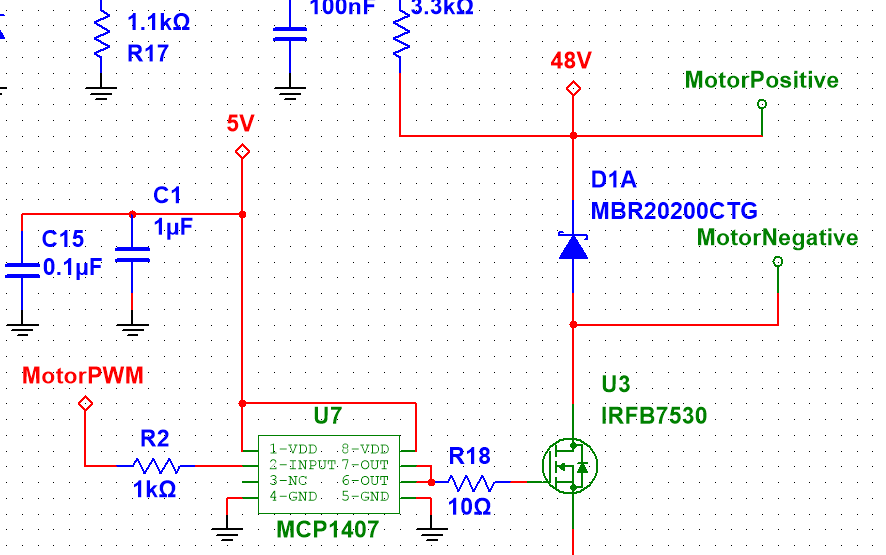
\includegraphics[width=0.85\linewidth]{Hardware/Pictures/Motorstyring}
	\caption{Motor controller hardware}
	\label{fig:Motorcontroller}
\end{figure}

\subsection{Implementation}
text

\subsection{Unity test}
text